\begin{frame}
        \frametitle{Synergistic Spent Nuclear Fuel Dynamics Within the European 
        Union}
\begin{itemize}
       \item Collaborative spent fuel management is materially feasible among nuclear
               nations in the  European Union.
       \item Collaborative EU spent fuel management could expedite a fast reactor
               technology transition in France.
       \item By using spent fuel from other EU nations, France can avoid
               building new light water reactors to support a transition to
               fast reactors.
\end{itemize}
\end{frame}


\begin{frame}
	\frametitle{Deployment Timeline for French Transition}
	110 SFRs (66 GWe) are deployed by 2076.
	\begin{figure}[htbp!]
	\begin{minipage}[b]{.45\linewidth}
        \begin{center}
                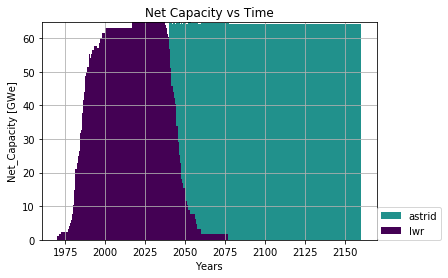
\includegraphics[width=\textwidth]{./images/french-transition/power_plot.png}
        \end{center}
        \caption{French Transition into an SFR Fleet}
        \label{fig:sfr_num}
	\end{minipage}
	\hspace{.5cm}
	\begin{minipage}[b]{.45\linewidth}
		\centering
		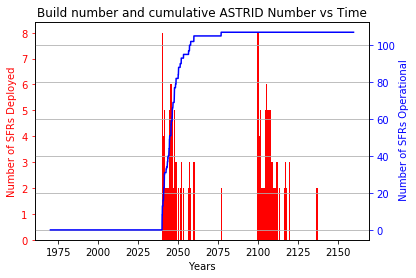
\includegraphics[width=\textwidth]{./images/french-transition/sfr_deploy.png}
		\caption{Deployment of French SFRs and total installed capacity}
		\label{fig:dep}
	\end{minipage}
\end{figure}
\end{frame}



\begin{frame}
\begin{figure}[htbp!]
    \begin{center}
        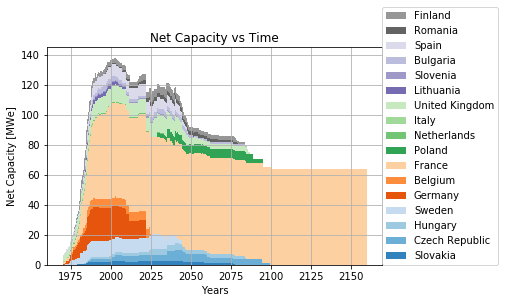
\includegraphics[width=\textwidth]{./images/onesim.png}
    \end{center}
    \caption{The simulated nuclear power deployment scheme relies on used
        nuclear fuel collaboration among nations.
        The historical operation of EU reactors is followed by the French transition to SFRs.  The steep transition from 2040 to 2060 reflects the scheduled decommissioning of reactors built in the 1975-2000 era of aggressive nuclear growth in France.}
    \label{fig:tot_dep}
\end{figure}
\end{frame}

